\headletter{W}
ithin this Chapter a few facets of the Internet of Things will be discussed, highlighting in particular its integration with and within semantic technologies. Over the Sections some actual implemented ideas will explain which are the benefits of adding the semantic layer, both with a SEPA dynamic background, and without.

In addition to this, in Section~\ref{sec:iomust} we will completely present the first major contribution of this Thesis, i.e., the Internet of Musical Things ontology. Its main goal is to open the way to collaborative musical production, with connected musical devices. Although it may appear that we address a limited subset of the whole IoT, Section~\ref{sec:iomust} will give proof that the methodology is on the contrary general and open for further enhancements.


%In particular, some references will be made on the contents of Chapter~\ref{ch:background}. The references will be compared with the works available in literature in Section~\ref{sec:31_rw}, and in two research projects: Arrowhead and Habitat (Sections~\ref{sec:arrowhead}, \ref{sec:habitat}). During their life-cycle these two projects were involved in a process that is still going on at various levels, from academy to hobbyists and makers, to enhance the panorama of IoT with new opportunities, both for technology and for users. 
%
%In addition to this in Section~\ref{sec:iomust} a new paradigm of IoT will be explored: the IoT for music, aiming to  A full desciption will be provided, resulting in one of the major contributions of this Thesis.

\section{Semantic Interoperability}
\label{sec:21_rw}

Chapter~\ref{ch:background} gave a broad view of the IoT panorama. The addition of semantics, as we said, could represent a technique to overcome vertical fragmentation. As a matter of fact, interoperability was one of the leading ideas since the first appearances of the Semantic Web concept \cite{berners2001semantic}.

But what does \textit{interoperability} actually means? As we said in Section~\ref{sec:iot}, from a technical point of view the term interoperability implies that there should be, among the considered systems, the same ISO-OSI stack. Consequently, interoperability should allow systems to be aware of the existence of other systems regardless of how they internally work. Furthermore, a successful exchange of requests should also be possible, including failure robustness.

Discovery mechanisms, for this reason, represent the bigger difference among interoperable and non interoperable systems: they allow agent-awareness and, if implemented at higher level, also successful communication feedback. Literature is rich, in this sense, and over the time provided a plethora of examples, middlewares and projects, some of which have been already cited. They, however, often operate in a closed environment, and mostly assume that parallel projects, whenever interested in a collaboration, should be reprogrammed to be compliant with their view.

The Semantic Web overcomes this required parallelism at information level as shown in Fig.~\ref{fig:honeycomb}. As it can be seen, the Semantic Internet of Things keeps its specific implementations, assumptions and realizations (the ``\texttt{app}'' boxes). However, while the incompatibilities in previous IoT were either not treated, or case by case solved with complex elaboration, we here transform it in semantic subgraphs that can coexist.
\begin{figure}
\centering
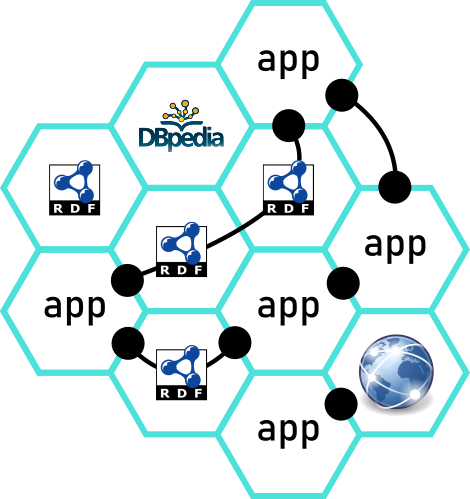
\includegraphics[scale=0.55]{honeycomb.png} 
\caption{Conceptual vision of the Semantic IoT. Local applications can directly communicate with each others, or with the Internet. Alternatively, they can share data through RDF formatting according to one or more ontologies.}
\label{fig:honeycomb}
\end{figure}

Consequently, interoperability is in this Section granted among collaborating systems relying on a continuous process of ontological inclusion. Such process was also targeted by previous research (e.g., \cite{halpin2010owl, calvanese2015ontology}). The Internet of Musical Things Ontology (see next Section) in this context provides a methodology to create such inclusion. The choice of a musical background, furthermore, is not limiting the suggested view: the core of the ontology, in other environments, is the common IoT universe (i.e. the \texttt{iot} namespace). The goal of Section~\ref{sec:iomust} is to setup an ontology by joining together other preexisting ontologies and taxonomies. Besides the innovative result materializing the IoMust in the Semantic Web panorama, one of the related outcomes is the interoperability achieved with IoMusT and any application made on top of the provided ontology components.

In Chapter~\ref{ch:semantic_wot}, in a different way, we will provide a broader view (but still semantically compatible with the present one), which includes also the web resources, unifying the Web and the IoT in the WoT over a semantic platform exploiting also SEPA.

\section{Internet of Musical Things}
\label{sec:iomust}
This Section takes inspiration from a recently submitted research paper: \faCopyright~~Turchet, L., Antoniazzi, F., Viola, F., Giunchiglia, F., \& Fazekas, G. (2019). The Internet of Musical Things Ontology. Submitted to~\textit{Journal of Web Semantics.}.

The Internet of Musical Things (IoMusT) is an emerging research area consisting of the extension of the Internet of Things paradigm to the musical domain. This field is positioned at the confluence of music technology, the Internet of Things, human-computer interaction, and artificial intelligence, and relates to the networks of computing devices embedded in physical objects (Musical Things) dedicated to the production and/or reception of musical content. Considering the computer science perspective, Turchet and colleagues \cite{turchet2018IoMusT} defined a Musical Thing as 
\begin{quote}
\textit{a computing device capable of sensing, acquiring, processing, or actuating, and exchanging data serving a musical purpose}
\end{quote} 
and defined the IoMusT as 
\begin{quote}
\textit{the ensemble of interfaces, protocols and representations of music-related information that enable services and applications serving a musical purpose based on interactions between humans and Musical Things or between Musical Things themselves, in physical and/or digital realms. Music-related information refers to data sensed and processed by a Musical Thing, and/or exchanged with a human or with another Musical Thing}
\end{quote}
  
Various kinds of Musical Things can be envisioned, which may be categorized according to the musical purpose they serve (e.g., to control, generate, or track responses to musical content). Examples of existing Musical Things are the ``smart musical instruments'', a new family of musical instruments encompassing sensors, actuators, wireless connectivity, and on-board processing \cite{turchet2019SMI}. These musical devices are able to directly exchange musically-relevant information with one another as well as communicate with a diverse network of external devices, such as smartphones, wearables, virtual reality headsets, or stage equipment. Instances of smart musical instruments include the Smart Caj\'{o}n reported in \cite{turchet_smartcajon_hit_2018} and the Sensus Smart Guitar developed by MIND Music Labs~\cite{turchet2017examples}. Another example of Musical Things are ``musical haptic wearables'' \cite{turchet_codesignMHW_2019}, a novel class of wearable devices embedding haptic stimulation, tracking of gestures and physiological parameters and wireless connectivity features. On the one hand, such devices were conceived to enhance communication between performers as well as between performers and audience members by leveraging the sense of touch in both co-located and remote settings. On the other hand, they were devised to enrich musical experiences of audiences of music performances by integrating haptic stimulations, as well as provide new capabilities for creative participation thanks to embedded sensor interfaces.  

Musical Things are connected by an infrastructure that enables multidirectional communication, both locally and remotely, between different stakeholders such as composers, performers, audience members, audio producers, live sound engineers, as well as music students and music teachers. The ecosystems that will form around Internet of Musical Things technologies are envisioned to support novel forms of interactions between such stakeholders by means of novel musical applications and services. This has the potential to revolutionize the way music is composed, performed, experienced, learned, and recorded. 

To accomplish the IoMusT vision, the Musical Things within an ecosystem need to dialog through a common language. A central unsolved issue within the IoMusT paradigm is how facilitating interoperability among heterogeneous Musical Things, which may serve radically different purposes (e.g., real-time analysis of musical content, generation and delivery of haptic, visual, or olfactory sensory layers additional to the musical content, delivery of content-recommendation services for music students). To date, interoperability across musical devices has mostly relied on protocols for the exchange of musical messages such as Musical Instrument Digital Interface (MIDI) or Open Sound Control (OSC) \cite{Wright2003OSC} and tools based on it (e.g., libmapper \cite{malloch2015distributed}). 

However, the existing musical protocols are not adequate to support interoperability across the wide heterogeneity of Musical Things, as they are typically not flexible, lack high resolution, not equipped with inference mechanisms, and do not support the integration with the Web. Semantic technologies, such as semantic web \cite{berners2001semantic} and knowledge representation \cite{sowa2000knowledge}, possess these features. For this reason, they have been recently envisioned as a solution to enable interoperability across heterogeneous Musical Things~\cite{turchet2018IoMusT}. Existing ontologies devised for the musical domain to date, such as the Music Ontology~\ontoref{music}, the Studio Ontology~\ontoref{studio} or the Audio Features Ontology~\ontoref{afo}, are insufficient to represent the wide knowledge base that the variety of the possible Musical Things entail. An ontology specific to the IoMusT scenario is currently missing. As a consequence, the use of semantic technologies in Internet of Musical Things contexts is limited to scenarios involving homogeneous Musical Things serving similar musical purposes or ad-hoc interactions designed for a specific, fixed scenario. 

The first effort towards the application of semantic technologies to the IoMusT context is reported in \cite{turchet2018sepa}. The authors proposed a semantically-enriched Internet of Musical Things architecture relying on a semantic audio server and edge computing techniques. Specifically, a SPARQL Event Processing Architecture \cite{roffia2018dynamic} was employed as an interoperability enabler allowing multiple Musical Things to cooperate, relying on a music-related ontology. A limitation of the developed architecture was the involvement of an ontology restricted to the representation of simple musical features, which prevented Musical Things dedicated to purposes other than music generation to join the ecosystem formed around the architecture.

Semantic technologies based on an ontology for the IoMusT can assist in managing, querying, and combining information characterizing an IoMusT ecosystem, including data about the music produced, the involved stakeholders, the utilized Musical Things and their application and services. This has the potential to spur the exploration of novel artistic avenues, such as performance and composition, for instance based on emergent properties of an IoMusT ecosystem \cite{ulieru2011emergent}. 

In this Section the ``Internet of Musical Things Ontology''~\ontoref{iomust} is exposed. The full design and evaluation process of the IoMusT Ontology is hereby given from the beginning to the current version, i.e., 1.0.0. The description of the IoMusT Ontology follows the MIRO (minimum information for the reporting of an ontology) guidelines~\cite{matentzoglu2018miro}. For reference, the paper reports the MIRO designations (e.g., E.9 for Ontology relationships), where the specific information item is provided. The ontology name (A.1) and its need (B.1) have been already introduced. The ontology is available on the web (see \ontoref{iomust}) (A.4) with license GPL3 (A.3).

\subsection{Methodology, audience, and scope}
This section describes the methodology adopted for the design and development of the IoMusT Ontology, as well as the audience of the ontology and its scope.

\subsubsection{\textsf{Methodology for ontology development}}
The ontology is developed and maintained by the authors and other members of the emerging IoMusT research community, which is currently composed by leading research institutes in sound music computing and Internet of Things (A.2 and C.2).

The design and development of the IoMusT Ontology was mostly inspired by the \textit{Methontology} methodological framework~\cite{fernandez1997methontology} (A.6). Such a framework is composed by six phases: i) the specification, i.e., the identification of the audience, scope, scenarios of use, and requirements; ii) the conceptualization of an informal model; iii) the formalization of the ontology namespaces, classes and properties; and iv) the integration of existing ontologies in a description and its reproduction in an OWL2 file \cite{motik2009owl}; v) the implementation of the ontology with an appropriate serialization language; vi) the maintenance of the ontology once implemented.

Moreover, the aforementioned framework identifies three tasks that are accomplished during the whole life of the ontology, which are orthogonal to the five phases: i) knowledge acquisition through research of related ontologies and models as well as gathering data from potential users), to inform multiple phases of the design process, mainly conceptualization and integration; ii) documentation of the process phases (internal) and the ontology specification (public); iii) the evaluation of the ontology before its release. 

Other works, like Uschold~\cite{uschold1996building} and more recently by De~Nicola et al.~\cite{de2016lightweight} suggest different methodologies for ontology engineering. These papers however include techniques that aim to formalize the setup from scratch of new ontologies. This is not the case in the current research, where the goal is to provide a new contribution based as much as possible on the integration of pre-existing contents.

\subsubsection{\textsf{Scope and audience}}
\label{ssec:audience_scope}
The role of the IoMusT Ontology is to offer a common data model enabling interoperability among heterogeneous Musical Things, which allows both people and virtual agents to seamlessly generate, explore, access, or transform music-related content produced within an IoMusT ecosystem. Therefore, the scope of the ontology (C.1) is represented by all ecosystems forming around existing or future IoMusT technologies.

The target audience of the ontology (B.3) is represented by all actors and stakeholders that are involved in such ecosystems, including performers, audience members, composers, studio producers, live sound engineers, and choreographers. 

\subsection{Related ontologies and data models}
\label{ssec:iomust_rw}
Before defining an ontology specific to the IoMusT domain we conducted a review of existing ontologies. The IoMusT vision is intrinsically multisensory and highly interdisciplinary \cite{turchet2018IoMusT}. This section describes ontologies and data models (B.2) that are related to such a vision. They have been gathered through the research of literature and online resources (D.1 and D.2) and evaluated as part of the design process (D.3).

\subsubsection{\textsf{Ontologies for the audio domain}}
Several ontologies have been proposed in recent years for the audio and music domains, in recognition of the complexity and broad ranging applications of such ontologies, and the fact that much of the information exchanged on the Web today is multimedia, of which music is a very substantial component, rather than text. The scope of such ontologies are wide ranging, starting from very focused areas of music production such as audio effects \cite{wilmering2013the}, to larger binding ontologies that target the description and retrieval of audio resources on the web in general \cite{ceriani2018audio}.

The Music Ontology (MO) \ontoref{music} \cite{raimond2007music, raimond2010spec} is a general purpose high-level ontology for the music domain that models the music value-chain from production to consumption. Therefore its focus is on editorial metadata, e.g. artist name and title associated with audio recordings, as well as the representation of major steps in the production of recorded music, from composition, through performance and recording, to release.

The Music Ontology does not deal with the nuances of technical workflows in music production. This is the area covered by the Studio Ontology \ontoref{studio} (SO) \cite{fazekas2011studio}. 

The Audio Features Ontology \ontoref{afo} (AFO) addresses another audio domain that requires detailed conceptualisations. Audio Features are descriptors that represent specific characteristics of sound signals. These may relate to measurable properties of the signal, such as bandwidth or spectral centroid, perceptual qualities like pitch and loudness, and musical characteristics such as notes, musical key and chords.

The Musical Instruments Ontology \cite{kolozali2011knowledge} is highly relevant to the domain of IoMusT. It provides an ontological model for encoding well known instrument classification systems, e.g. for grouping instruments into categories such as \textit{Idiophones} or \textit{Aerophones}, based on their sound production or excitation mechanism.

The Audio Commons Ontology (ACO) \ontoref{aco} \cite{ceriani2018audio} is an example of a higher level domain ontology that binds several audio related ontologies together. It was designed to facilitate the integration of audio content repositories on the Web as well as content consumption by software agents. 

\subsubsection{\textsf{Ontologies for sensors, actuators and connectivity}}
Among the ontologies designed for the IoT, two of the most diffuse are SSN (Semantic Sensor Network) and SOSA (Sensor, Observation, Sample, and Actuator) \ontoref{ssn, sosa}. Both SSN and SOSA adopt a complex approach to description of hardware, observation of physical entities and actuation. SSN~\cite{compton2011ssn} covers the majority of the SensorML standard\footnote{\faLink~\url{https://www.opengeospatial.org/standards/sensorml}} and has been designed to describe sensors and observations, as well as the deployment in which sensors are employed. SOSA~\cite{janowicz2018sosa} adopts a lightweight approach to describe sensors, actuators and the acts of observation and actuation. SOSA acts as a replacement of the Sensor-Stimulus-Observation (SSO) design pattern provided by SSN, that provides greater expressivity~\cite{haller2018sosa}.

At a higher level of abstraction, things in IoT can be represented according to the Web Thing model\footnote{\faLink~\url{https://www.w3.org/Submission/wot-model/}} proposed by the W3C. In this sense, devices are provided with the so-called thing description, a detailed profile reporting properties, events and actions exposed through its interface. A first attempt to semantically represent this model has been provided by Charpenay et al. in~\cite{charpenay2016introducing}, later on envisioned by Serena et al. in~\cite{serena2018discovery} for a discovery framework. The Web of Things ontology discussed by Charpenay et al. and Serena et al. has been employed by Viola et al.~\cite{viola2018playsound} to build a semantic Web of Things enviroment for recommendations in the audio domain. Eventually, Antoniazzi et al.~\mbox{\cite{antoniazzi2019building}} provided a semantic version of the Web of Things.

\subsection{Specification}
\label{ssec:specification}
The acquired knowledge was then analzed to identify a set of requirements that the ontology should satisfy \cite{siegemund2011towards}. The literature review led to a total of 15 scenarios (5 scenarios from \cite{turchet2018IoMusT}, 5 from \cite{turchet2019SMI}, and 5 defined by the authors or derived from recent experiments with users described in the literature). For each scenario we derived a set of requirements, and then applied a thematic analysis \cite{BraCla06} to reduced them. The resulting requirements are represented below as a list of example questions that the ontology should be able to support answering \cite{gruninger1995methodology}, and a list of formal requirements.


\subsubsection{\textsf{Competency questions}}
The following sample questions are meant to be asked with respect to an IoMusT ecosystem:
\begin{multicols}{2}
\begin{enumerate}
\item Which type of Musical Things are used by the local and remote performers during the live concert?
\item How many Musical Things used by the audience provide haptic feedback?
\item What smart instruments are controlling the smartphones used by the audience?
\item What is the mood of the music at a given time during the live performance?
\item How many audience members are actively participating to the music creation process thanks to their Musical Things?
\item Which kind of stage equipment is used at a given time during the concert?
\item Which gestural and biometric parameters are tracked from the audience during the live performance?
\item How many and which kind of networks are used during a performance?
\item Which pedagogical applications are available for a smart violin?
\item With which music content repository a smart ukulele can interact?
\item Which services are available for a smart guitar and what are their purposes?
\item What type of sensors and actuators compose a smart musical instrument or a musical haptic wearable?
\end{enumerate}
\end{multicols}

\subsubsection{\textsf{Formal requirements}}
The IoMusT Ontology should be able to:
\begin{multicols}{2}
\begin{enumerate}

\item represent the concept of Musical Things, including: 
	\begin{enumerate}[wide, labelindent=0pt]
	\item its type (e.g., musical instrument, wearable device, stage equipment);
	\item its characteristics including the number and type of inputs (e.g., sensors tracking movements or biometric parameters) and outputs (e.g., auditory, visual, haptic, olfactory);
	\item the type of person for which it is conceived (e.g., performer, audience member, live sound engineer, producer); 
	\item its function (e.g., a smart instrument used to produce musical content, a musical haptic wearable aiming at enriching the listeners' musical experience, an interface used by audience members for participatory purposes, a device used to infer the mood of audience members based on sensed quantities);
	\item its geographical position;
	\item the type of data that it generates (e.g., audio signal, text message);
	\end{enumerate}
	
\item represent the concept of connectivity, including: 
	\begin{enumerate}[wide, labelindent=0pt]
	\item the type of network involved (e.g., local network, remote network, Wi-Fi-based, millimeter waves-based);
	\item the attributes of the network (e.g., bandwidth, speed, synchronization mechanisms);
	\item the time taken by the network to deliver/receive a message to/from a certain Musical Thing;
	\end{enumerate}

\item represent the concept of application and service, including:
	\begin{enumerate}[wide, labelindent=0pt]
	\item its purpose (e.g., for music learning, performance, composition, studio production)
	\item its level of interactivity (e.g., interactive, non-interactive)
	\item its type (e.g., social network, online music content repository)
	\item its user (e.g., composer, performer, studio producer, educationalist, student, audience member)
	\end{enumerate}

\item describe attributes of the music (produced live) at a given time, including:
	\begin{enumerate}[wide, labelindent=0pt]
	\item low-level features (e.g., the density of notes);	
	\item high-level features (e.g., the mood)
	\end{enumerate}	
	
\item describe attributes of the ecosystems, including:
	\begin{enumerate}[wide, labelindent=0pt]
	\item the number and type of Musical Things present in the network at a given time and a given space;
	\item which Musical Things are interacting;
	\item the number and type of applications and services available within the ecosystem; 
	\item the number and type of networks used at a given time.
	\end{enumerate}	

\end{enumerate}
\end{multicols}

\subsection{Ontology description}
\label{ssec:description}
The Internet of Musical Things ontology (the IoMusT Ontology) has been developed incrementally. As a matter of fact, the task of developing ontologies is in general complex, and needs an approach that involves continuous refinement and check of concepts and relationships. This can be done in several ways, and may be performed iteratively as long as the expected match of the ontology with the real subject is achieved. 

Not surprisingly, the first step is to split the domain of interest in smaller parts if possible. For each of those smaller parts, secondly, iterations are needed to ensure that all relevant concepts are included. Sometimes this is done by surveying a pool of experts and/or future users of the ontology, to get their feedback. Clearly, this check helps designers to avoid wrong naming on resources, as well as to detect and correct contradictory assertions.

Then, the smaller parts have to be joined together to form the ontology. Again, the expressiveness of the complete work has to be checked, and in this paper this is provided by requirement analysis and evaluation. The question to be answered, here, is: \textit{is my ontology capable to describe my context? If so, is the description made with the precision needed?} This process also may be performed iteratively.

IoMusT Ontology is not an exception. On the contrary, it is very important to notice that the formalization of a vocabulary for Internet of Musical Things needs this feedback process to ensure a coherent representation of music-related entities with general-purpose contents. 

A bottom-up process was deployed for our case. In particular, jumping from wider to narrower concepts, the first idea to be discussed is indeed the connection that stands between the global interpretation of Internet of Things and how to decline it into the Internet of Musical Things. See also Fig.~\ref{fig:fig1}. Clearly, the former is larger than the latter, which should represent a specialization and rely on it. The usage of the IoMusT Ontology, as a consequence, should allow a transparent view of any Musical Thing context as an IoT system. There would be no point in ignoring this core aspect, because the core idea of ontology engineering is to provide a shared and interoperable way to collaborate between different fields of knowledge. Any design choice opposed to this view would have as a direct result the creation of another vertical silos within the IoT chaos \cite{broring2017enabling}.

In order to replicate in the ontology this necessary duality, this work will suggest the adoption of two new namespaces:
\begin{enumerate}
    \item \texttt{iot}, that will be used to connect concepts that belong to the broader view of generic devices;
    \item \texttt{iomust}, which is an extension of \texttt{iot} defined as \texttt{iot:musical}. Within this namespace are organized the concepts of music-related IoT;
\end{enumerate}

For the sake of clarity the prefixes are kept in a contracted form. To see their expanded version, please see the \hyperref[sec:ontology_list]{List of Ontologies}.

\subsubsection{\texttt{iot} \textsf{namespace}}

The first concept to be defined is the \textit{Thing} as it is intended in the acronym IoT. Liu et al.~\cite{liu2016comparison} survey and comment the spectrum of definitions that have been suggested in literature over the time. Among the surveyed entries, the one proposed by the IEEE is coherent with our requirement of generality: the thing 
\begin{quote}
\textit{is any physical object relevant from a user or application perspective}
\end{quote} 
meaning that we consider things as items exploiting, or being exploited by, other items. Therefore, from now on, the class \texttt{iot:Thing} has to be considered according to this definition. Notice that also regular everyday life objects may be \texttt{iot:Thing}s, like chairs, pillows, a scarf, a painting and, indeed, a musical instrument.

Clearly, this is a generic class that needs to be further specialized in subclasses. Again, a lot of help can come from the listings in \cite{liu2016comparison}, as \texttt{iot:Thing} is definitely a huge container. For instance, things can be wearable objects: so, the class \texttt{iot:WearableThing} can be defined to represent this category. Similarly, devices can also be \textit{smart}, so we call for \texttt{iot:SmartThing} class: smart things, e.g., a smartphone, a smart TV, include special technological features or artifacts that provide them with relevant added value over the basic version of the same object. 

Eventually, things can be connected to a communication network: they are, in this case, instances of the class \texttt{iot:ConnectedThing}. Notice that the aforementioned Studio Ontology \ontoref{studio} contains a rich environment of properties and classes related to connectivity (e.g., the \textit{Connectivity} and the \textit{Device} sub-ontologies). %Fully including it in the IoMusT Ontology is a task that goes beyond the scope of this paper, but still it is a future project, as it may be a direct answer to some competency question & requirements.

It would neither be reasonable, nor useful, to list here a hundred of possible subclasses. For this reason, in the present paper only a few will be defined, as the discussion requires them. It is important to notice that there is complete freedom to include new classes whenever needed, as this is precisely the kind of incremental approach for ontology engineering which was above aforementioned.

\subsubsection{\textsf{Musical things in the \texttt{iomust} namespace}}

IoMusT Ontology, as already said, aims to develop the \texttt{iot} namespace in its musical flavour. To do so, the reference to a vocabulary connected to music is essential. Our reference in this work was introduced in Section~\ref{ssec:iomust_rw}: it is the Music Ontology~\ontoref{music}, which will be mentioned as the \texttt{music} namespace. An important contribution of this namespace in IoMusT Ontology is its supporting role in creating the archetype of Musical Thing, i.e. the class \texttt{iomust:MusicalThing}. In the present work, our definition for this class is the following: the Musical Thing is \textit{a thing used to produce or enjoy music, with reference to its context}. As a consequence, IoMusT Ontology will consider that a smart loudspeaker, a CD by David Bowie belong to that class, as well as a smart violin located in a concert hall. The same smart violin, however, if stored for exposition in a museum, is no more an \texttt{iomust:MusicalThing} because it loses its musical production interest. 

The class \texttt{iomust:MusicalThing} is indeed less generic than its superclass \texttt{iot:Thing}, because it provides a light form of contextualization. Yet, however, we need more precise solutions to be even less abstract. All the items identified in the example above (the smart loudspeaker, the CD, the smart violin) would point to \texttt{iot:Thing} through the \texttt{rdf:type} predicate. Then, to include an explicit reference to music, and introduce the Internet of Musical Things namespace, the following rule applies:
\begin{rul}
\label{rule:musical_thing}
    If an \texttt{iot:Thing} instance is also connected through \texttt{rdf:type} to a class belonging to the Music Ontology, then it is also an instance of \texttt{iomust:MusicalThing}. 
\end{rul}
A typical application of Rule~\ref{rule:musical_thing} is the aforementioned smart violin:  consider Expression~\ref{listing:violin_1} as an example, where a simple triple representation is given of the implication expressed. Notice that Rule~\ref{rule:musical_thing} is not intended to be strictly reversible: during a concert, lights and smoke machines may be intended as Musical Things because of their essential contribution to the listening experience, and yet may not be included in one of the \texttt{music} namespace categories. 
\begin{multline}
\label{listing:violin_1}
\texttt{ns:SmartViolin a iot:Thing, music:Instrument} \\ \Rightarrow \texttt{ns:SmartViolin a iomust:MusicalThing}
\end{multline}

%\begin{lstlisting}[caption={Triple representation of Rule~\ref{rule:musical_thing}. Extended prefixes are available in Table~\ref{tab:prefixes}.}, label={listing:violin_1}, mathescape]
%ns:SmartViolin a iot:Thing, music:Instrument
%$\Rightarrow$
%ns:SmartViolin a iomust:MusicalThing
%\end{lstlisting}
The Generic Musical Thing definition is not enough to build the complete IoMusT. Here it follows a sequence of new classes to be introduced in the \texttt{iomust} environment, descending from the Musical Thing. Each of the classes here corresponds to a rule similar to Rule~\ref{rule:musical_thing} in the OWL.
\begin{description}[wide, labelindent=0pt]
\item[\texttt{iomust:SmartMusicalThing}] is a Musical Thing that is also an \texttt{iot:SmartThing};
\item[\texttt{iomust:SmartInstrument}] is a Musical Thing that is also a \texttt{music:Instrument};
\item[\texttt{iomust:WearableMusicalThing}] is a Musical Thing that is also an \texttt{iot:WearableThing};
\item[\texttt{iomust:StageEquipment}] is a collection of Musical Things serving as equipment. The definition of collection can be extracted from external ontologies designed \textit{ad hoc} for this, like \ontoref{collection}.
\end{description}

Table~\ref{tab:musical_thing_examples} contains some practical examples of usage for the \texttt{iot} and \texttt{iomust} namespace entities.

\begin{table*}[t]
    \centering \footnotesize
    \caption{Example of usage for \texttt{iot} and \texttt{iomust} namespaces. We here show how objects part of an Internet of (Musical) Things environment can be considered instances of the classes introduced in this research. Extended prefixes are available in the \hyperref[sec:ontology_list]{List of Ontologies}.}
    \label{tab:musical_thing_examples}
    \vspace{3mm}
    \begin{tabular}{r|c|c|c|c|c|c|c|c|c|}
     & \rotatebox{90}{\texttt{ns:Bob}} & \rotatebox{90}{\texttt{ns:Wardrobe}} & \rotatebox{90}{\texttt{ns:SmartCar}} & \rotatebox{90}{\texttt{ns:Violin}} & \rotatebox{90}{\texttt{ns:SmartViolin}} & \rotatebox{90}{\texttt{ns:TShirt}} & \rotatebox{90}{\texttt{ns:StageLight}} & \rotatebox{90}{\texttt{ns:VR\_HeadSet}} &
     \rotatebox{90}{\begin{tabular}{@{}c@{}}\texttt{ns:HeartBeatSensor} \\ for music experiment \end{tabular}} \\
     \hline
    \texttt{foaf:Person} & \faCheck  &  &  &  &  &  &  &  &\\ \hline
    \texttt{iot:Thing} &  &  \faCheck &  \faCheck & \faCheck  & \faCheck & \faCheck  & \faCheck  & \faCheck & \faCheck \\ \hline
    \texttt{iot:SmartThing} &  &  &  \faCheck &  &  \faCheck &  & \faCheck & \faCheck & \\ \hline
    \texttt{iot:ConnectedThing} &  &  &  &  &  \faCheck &  & \faCheck & \faCheck & \faCheck \\ \hline
    \texttt{iot:WearableThing} &  &  &  &  & & \faCheck &  &  \faCheck & \faCheck \\ \hline
    \texttt{music:Instrument} &  &   &  & \faCheck &  \faCheck &  &  &  & \\ \hline
    \texttt{iomust:MusicalThing} &  &   &  & \faCheck  &  \faCheck &  &  \faCheck &  & \faCheck \\ \hline
    \texttt{iomust:SmartMusicalThing} & &  &   &  &  \faCheck &  & \faCheck  &  & \\ \hline
    \texttt{iomust:SmartInstrument} &  &  &  &  &  \faCheck &  &  &  & \\ \hline
    \texttt{iomust:StageEquipment} item &  &  &  &  &  &  & \faCheck &  &  \\ \hline
    \texttt{iomust:WearableMusicalThing} &  &  &  &  &  &  &  &  & \faCheck\\ \hline
    \end{tabular}
\end{table*}

\subsubsection{\textsf{\texttt{iot} \& \texttt{iomust} sensing, actuating and interacting}}
So far the discussion on the IoMusT Ontology was conducted as a set of broad definitions for the baseline concepts. Here, instead, space is given to how the integration of other ontologies enables our vision of  the IoMusT from a lower level standpoint.

First of all it is necessary to describe the smart devices more in detail, and include additional information related to the electronic devices embedded in the \texttt{iot:Thing} (e.g., micro-controllers, sensors, actuators). The \texttt{iot:SmartThing} was previously introduced to this effect, though without any other specificity. Consequently, to provide greater precision on the actual available sensing and actuating units, other information is needed. Taking into  consideration Table~\ref{tab:musical_thing_examples} as an example, we have to provide a way to semantically distinguish between two instances of \texttt{iot:SmartThing}, like the smart violin, and the virtual reality headset, based on their setup. To achieve such goal, this work suggests the inclusion of an ontology already existing and well known in the panorama, namely, SOSA \ontoref{sosa}. The choice of SOSA has three main advantages that greatly benefit IoMusT Ontology: (i) SOSA is \textit{de facto} a light version of SSN, and therefore the IoMusT Ontology can be furtherly extended towards SSN integration very easily; (ii) SOSA is very simple, which is always a relevant factor when studying, building and integrating ontologies; (iii) SSN and SOSA, eventually, are a relatively recent W3C recommendation (the last draft dates back to 2017), which means that they are globally accepted as a reference.

The realization of this ontological alignment is made by including as a plug-in the concept of \texttt{sosa:Platform} in the IoMusT Ontology subgraph for the \texttt{iot:Thing} and its aforementioned subclasses. According to SOSA documentation, the \texttt{sosa:Platform} is an \textit{entity that hosts other entities, particularly Sensors, Actuators, Samplers, and other Platforms}, that is precisely the facet missing until now in the \texttt{iot} namespace. In 
%Listing~\ref{listing:sosa_example} 
Fig.~\ref{graph:sosa_example}
a few examples are provided to show how the connection can be made. As it can be seen, the smart guitar instance \texttt{ns:SmartGuitar} has also as \texttt{rdf:type} the \texttt{sosa:Platform} class. This additional type allows us to include references to the sensors and actuators on board, as well as the entity they measure. Further details on sensing and measurement description, extensively discussed in previous researches like \cite{rijgersberg2013ontology, narock2009using} and surveyed in \cite{wang2015survey}, are out of the scope of this paper. For the future, anyway, the possibility to integrate new ontologies still exists: for the ones exploiting SOSA and SSN, such process should be trivial.

\begin{figure*}[h!]
\begin{center}
\begin{tikzpicture}[->,>=stealth']

\node[state,draw=mauve!90,fill=mauve,text=white,align=center] (SMARTGUITAR) {
\begin{tabular}{l}
  \parbox{2.6cm}{\texttt{ns:SmartGuitar}}
   \end{tabular}
};
  
 % State: ACK with different content
 \node[state,  yshift=2.4cm, right of=SMARTGUITAR, node distance=3cm, anchor=center, draw=yellow!90,fill=yellow!90,align=center] (SGTYPES) {%
    \begin{tabular}{l} 
        \parbox{4.8cm}{\texttt{iot:Thing, sosa:Platform, iot:SmartThing, iomust:MusicalThing, music:Instrument, iomust:SmartInstrument, iomust:SmartMusicalThing;}}
    \end{tabular}
};
  
   % State: ACK with different content
\node[state, yshift=0cm, right of=SMARTGUITAR, node distance=6.5cm, anchor=center, draw=mauve!90,fill=mauve!90,align=center,text=white] (IMUSENSOR) {%
    \begin{tabular}{l}
        \parbox{2.2cm}{\texttt{ns:IMUSensor}}
    \end{tabular}
};
  
\node[state, yshift=-1.5cm, right of=SMARTGUITAR, node distance=5cm, anchor=center, draw=mauve!90,fill=mauve!90,align=center,text=white] (CONTACTMIC) {%
    \begin{tabular}{l} 
        \parbox{3.8cm}{\texttt{ns:ContactMicrophone}}
    \end{tabular}
};
  
\node[state, yshift=-3cm, right of=SMARTGUITAR, node distance=1cm, anchor=center, draw=mauve!90,fill=mauve!90,align=center,text=white] (LOUDSPEAKER) {%
    \begin{tabular}{l} 
        \parbox{2.6cm}{\texttt{ns:Loudspeaker}}
    \end{tabular}
};
  
\node[state, yshift=0cm, right of=IMUSENSOR, node distance=4cm, anchor=center, draw=yellow!90,fill=yellow!90,align=center] (SENSORS) {%
    \begin{tabular}{l}
        \parbox{2cm}{\texttt{sosa:Sensor}}
    \end{tabular}
};
  
\node[state, yshift=0cm, right of=LOUDSPEAKER, node distance=5cm, anchor=center, draw=yellow!90,fill=yellow!90,align=center] (ACTUATORS) {%
    \begin{tabular}{l}
        \parbox{2.4cm}{\texttt{sosa:Actuator}}
    \end{tabular}
};
  
\node[state, yshift=0cm, right of=SGTYPES, node distance=5.5cm, anchor=center, draw=mauve!90,fill=mauve!90,align=center,text=white] (IMUHOSTS) {%
    \begin{tabular}{l} 
        \parbox{3cm}{\texttt{ns:Acceleration, ns:Rotation, ns:Orientation}}
    \end{tabular}
};
  
\node[state, yshift=-1.3cm,  right of=IMUHOSTS, node distance=3.5cm, anchor=center, draw=yellow!90,fill=yellow!90,align=center] (OBSERVABLEPROPERTY) {%
    \begin{tabular}{l} 
        \parbox{4.4cm}{\texttt{sosa:ObservableProperty}}
    \end{tabular}
};
  
\node[state, yshift=0cm, right of=CONTACTMIC, node distance=6.7cm, anchor=center, draw=mauve!90,fill=mauve!90,align=center,text=white] (VIBRATION) {%
    \begin{tabular}{l}
        \parbox{2.2cm}{\texttt{ns:Vibration}}
    \end{tabular}
};
  
\node[state, yshift=-1cm,  right of=LOUDSPEAKER, node distance=4cm, anchor=center, draw=mauve!90,fill=mauve!90,align=center,text=white] (SOUND)  {%
    \begin{tabular}{l} 
        \parbox{1.4cm}{\texttt{ns:Sound}}
    \end{tabular}
};
  
\node[state, yshift=0cm, right of=SOUND, node distance=5cm, anchor=center, draw=yellow!90,fill=yellow!90,align=center] (ACTUATABLEPROPERTY) {%
    \begin{tabular}{l}
        \parbox{4.4cm}{\texttt{sosa:ActuatableProperty}}
    \end{tabular}
};
 
\path (SMARTGUITAR)     edge[bend left=30,draw=blue]  node[anchor=north,above]{\textcolor{blue}{\texttt{a~~}}}   (SGTYPES)
(SMARTGUITAR)   edge[anchor=south,draw=blue] node[]{\textcolor{blue}{\texttt{sosa:hosts}}}                      (IMUSENSOR)  
(SMARTGUITAR)   edge[bend right=10,draw=blue] node[anchor=south, below]{\textcolor{blue}{\texttt{sosa:hosts}}}  (LOUDSPEAKER)  
(SMARTGUITAR)   edge[bend right=20,draw=blue] node[anchor=south, above]{\textcolor{blue}{\texttt{sosa:hosts}}}  (CONTACTMIC)
(IMUSENSOR)     edge[draw=blue] node[anchor=north]{\textcolor{blue}{\texttt{a}}}                                (SENSORS)
(LOUDSPEAKER)   edge[draw=blue] node[anchor=north]{\textcolor{blue}{\texttt{a}}}                                (ACTUATORS)
(CONTACTMIC)    edge[draw=blue] node[anchor=north]{\textcolor{blue}{\texttt{a}}}                                (SENSORS)
(IMUSENSOR)     edge[draw=blue] node[]{\textcolor{blue}{\texttt{sosa:observes}}}       (IMUHOSTS)
(IMUHOSTS)     	edge[bend left=30,draw=blue] node[anchor=north]{\textcolor{blue}{\texttt{a}}}                                (OBSERVABLEPROPERTY)
(CONTACTMIC)    edge[draw=blue] node[anchor=north]{\textcolor{blue}{\texttt{sosa:observes}}}                    (VIBRATION)
(VIBRATION)     edge[bend right=30, draw=blue] node[anchor=north]{\textcolor{blue}{\texttt{~~a}}}                                (OBSERVABLEPROPERTY)
(LOUDSPEAKER)   edge[bend right=10, draw=blue] node[below]{\textcolor{blue}{\texttt{sosa:actsOnProperty~~~~~~~~~~~~}}}         (SOUND)
(SOUND)     	edge[draw=blue] node[anchor=north, below]{\textcolor{blue}{\texttt{a}}}                                (ACTUATABLEPROPERTY);   

\end{tikzpicture}
\end{center}
\caption{SOSA integration with the IoMusT Ontology. Extended prefixes are available in the \hyperref[sec:ontology_list]{List of Ontologies}. The color scheme is the same used in Prot\'eg\'e \cite{protege}.\\Legend:~~\textbf{\textcolor{yellow!90}{Classes}~~\textcolor{mauve!90}{Individuals}~~\textcolor{blue}{Object Properties}}.}
\label{graph:sosa_example}
\end{figure*}

Sensing and actuating are in general part of a greater intent of interactive IoT system design. Data collection, then, provides the tools to create a feedback to control actuation and, eventually, to show smart behavior. Interaction is an unavoidable part of this process and, consequently, it should also be represented in the ontology alongside with sensors and actuators. Once such semantic prototype is given, it is possible to distinguish the active resources from the environmental passive ones and an interaction is finally possible. Besides, if the semantic view is shared among various systems horizontally, a strong and effective interoperability is automatically achieved.

The study of entities interacting within their environment is a well established field in literature, leveraging the concepts of \textit{agent} (e.g., \cite{jennings1999agent, leitao2016smart, kravari2015survey} and many others) and \textit{semantic agent} (see, for instance, \cite{hendler2001agents, lin2010modeling}). 

Within the IoMusT Ontology, the agent is referred to as any entity, human, object or virtual, that is capable of triggering any kind of dynamic evolution in an environment populated by instances of \texttt{iot:Thing} class. Both \texttt{iot} and \texttt{iomust} namespaces do not include directly such content, as their focus is the device, regardless the interaction aspect. For this reason, and for the discussion above, the IoMusT Ontology needs to rely on external ontologies to properly provide a definition of agent. Similarly to what has been suggested in the previous paragraphs with SOSA, we suggest here to exploit well-known ontologies, namely \ontoref{foaf} and \ontoref{prov}. 

The former, once connected to the IoMusT Ontology, defines the \texttt{foaf:Agent} as \textit{person, group, software or physical artifact}, and \textit{things that do stuff}. The idea of agent suggested in the previous paragraph is clearly derived from FOAF, although its real utility, in our research, is its capability of including the human being class \texttt{foaf:Person} and relationships in the semantic environment. Agents, intended as physical and virtual devices, are described through the latter, PROV-O, where the agent is \textit{something that bears some form of responsibility for an activity taking place, for the existence of an entity, or for another agent's activity} \cite{lebo2013prov}. This idea, in particular, includes also entities running software, which belong to \texttt{prov:SoftwareAgent}. Listing~\ref{listing:foaf_example} shows an example of using FOAF and PROV-O, and introduces in the \texttt{iot} namespace the ownership property \texttt{iot:owns}. 
\begin{lstlisting}[caption={FOAF \& PROV-O integration with the IoMusT Ontology. Extended prefixes are available in Table~\ref{tab:prefixes}.}, label={listing:foaf_example}]
ns:cristina     a   		foaf:Agent, foaf:Person, 
                    		prov:Agent, prov:Person;
                foaf:name 	'Cristina';
                iot:owns  	ns:SmartGuitar.
\end{lstlisting}
Ownership and actual usage do not necessarily coincide: it may happen, for instance, that people use a tool belonging to someone else. Besides, ownership does not imply any sort of activity with the device. A setup for activities, part of the IoMusT Ontology, is available in Fig.~\ref{graph:activities}.

\begin{figure*}[!ht]
\begin{center}
\begin{tikzpicture}[->,>=stealth']

\node[state,draw=mauve!90,fill=mauve!90,text=white,align=center] (BOB) {
\begin{tabular}{l}
  \parbox{1.1cm}{\texttt{ns:bob}}
   \end{tabular}
};
  
 % State: ACK with different content
 \node[state,  yshift=2cm, right of=BOB, node distance=4cm, anchor=center, draw=yellow!90,fill=yellow!90,align=center] (BOBTYPES) {%
    \begin{tabular}{l} 
        \parbox{3cm}{\texttt{foaf:Agent, foaf:Person, 
                music:Performer, prov:Agent, prov:Person;}}
    \end{tabular}
};

 % State: ACK with different content
 \node[state,  yshift=2cm, node distance=0cm, anchor=center, draw=green!90,fill=green!90,align=center] (BOBNAME) {%
    \begin{tabular}{l} 
        \parbox{0.9cm}{\texttt{'Bob'}}
    \end{tabular}
};
  
   % State: ACK with different content
\node[state, yshift=-2cm, anchor=center, draw=mauve!90,fill=mauve!90,align=center,text=white] (CRISTINA) {%
    \begin{tabular}{l}
        \parbox{2.1cm}{\texttt{ns:cristina}}
    \end{tabular}
};
  
\node[state, right of=BOB, node distance=6.9cm, anchor=center, draw=mauve!90,fill=mauve!90,align=center,text=white] (APPLICATION) {%
    \begin{tabular}{l} 
        \parbox{3.8cm}{\texttt{ns:IomustApplication}}
    \end{tabular}
};

 \node[state, right of=BOBTYPES, node distance=6cm, anchor=center, draw=yellow!90,fill=yellow!90,align=center] (APPLICATIONTYPES) {%
    \begin{tabular}{l} 
        \parbox{6cm}{\texttt{iot:Application, prov:Activity,
        iomust:MusicalThingApplication;}}
    \end{tabular}
};

\node[state, yshift=-1cm ,draw=mauve!90,right of=APPLICATION, node distance=5cm, fill=mauve!90,text=white,align=center] (SMARTGUITAR) {
\begin{tabular}{l}
  \parbox{2.6cm}{\texttt{ns:SmartGuitar}}
   \end{tabular}
};

\node[state,yshift=-1cm, 
%draw=purple!90,
right of=CRISTINA, node distance=6.5cm, 
%fill=purple!90,
%text=white,
align=center] (EVENT) {
\begin{tabular}{l}
  \parbox{1.2cm}{\texttt{\_:event}}
   \end{tabular}
};

 \node[state,  yshift=-1.5cm, right of=CRISTINA, node distance=12cm, anchor=center, draw=yellow!90,fill=yellow!90,align=center] (EVENTTYPES) {%
    \begin{tabular}{l} 
        \parbox{3.4cm}{\texttt{event:Event, prov:Entity, music:Performance;}}
    \end{tabular}
};

\node[state,yshift=-3cm, 
%draw=purple!90,
right of=CRISTINA, node distance=6.5cm,
%fill=purple!90,
%text=white,
align=center] (EVENTTIME) {
\begin{tabular}{l}
  \parbox{2cm}{\texttt{\_:eventtime}}
   \end{tabular}
};

\node[state,yshift=0cm, 
draw=yellow!90,fill=yellow!90,align=center,
right of=EVENTTIME, node distance=5cm,
align=center] (EVENTTIMETYPE) {
\begin{tabular}{l}
  \parbox{3.2cm}{\texttt{timeline:Interval}}
   \end{tabular}
};

 \node[state,  yshift=-3cm, right of=BOB, node distance=1cm, anchor=center, draw=green!90,fill=green!90,align=center] (STARTTIME) {%
    \begin{tabular}{l} 
        \parbox{4.1cm}{\texttt{'2019-06-18T12:00:00Z'}}
    \end{tabular}
};

 \node[state,  yshift=-5cm, node distance=0cm, anchor=center, draw=green!90,fill=green!90,align=center] (DURATION) {%
    \begin{tabular}{l} 
        \parbox{1cm}{\texttt{'PT1H'}}
    \end{tabular}
};
 
\path (BOB)     edge[draw=blue]  node[anchor=south,above]{\textcolor{blue}{\texttt{a}}}   (BOBTYPES)
(BOB)     edge[draw=green]  node[anchor=south,above]{\textcolor{green}{\texttt{foaf:name}}}   (BOBNAME)
(BOB)   edge[draw=blue] node[]{\textcolor{blue}{\texttt{foaf:knows}}}                      (CRISTINA)  
(BOB)   edge[draw=blue] node[anchor=south, above]{\textcolor{blue}{\texttt{iot:isInvolvedIn}}}  (APPLICATION)  
(APPLICATION)   edge[draw=blue] node[anchor=south, above]{\textcolor{blue}{\texttt{a}}}  (APPLICATIONTYPES)
(SMARTGUITAR)     edge[bend right=10, draw=blue] node[anchor=west]{\textcolor{blue}{\texttt{iot:isInvolvedIn}}} (APPLICATION)
(APPLICATION)   edge[draw=blue] node[text width=2cm]{\textcolor{blue}{\texttt{iot:produces,\\ prov:generated}}}                                (EVENT)
(EVENT)   edge[draw=blue] node[anchor=south west, text width=2cm]{\textcolor{blue}{\texttt{a}}}                                (EVENTTYPES)
(EVENT)   edge[draw=blue] node[text width=2cm]{\textcolor{blue}{\texttt{event:agent}}}                                (BOB)
(EVENT)   edge[bend right=10, draw=blue] node[text width=2cm]{\textcolor{blue}{\texttt{event:factor}}}                                (SMARTGUITAR)
(EVENT)   edge[draw=blue] node[anchor=south,text width=2cm]{\textcolor{blue}{\texttt{event:time}}}                                (EVENTTIME)
(EVENTTIME)   edge[draw=blue] node[anchor=south]{\textcolor{blue}{\texttt{a}}}                                (EVENTTIMETYPE)
(EVENTTIME)   edge[bend left=20,draw=green] node[anchor=south,text width=2cm]{\textcolor{green}{\texttt{timeline:start}}}                                (STARTTIME)
(EVENTTIME)   edge[draw=green] node[anchor=north]{\textcolor{green}{\texttt{timeline:duration}}}                                (DURATION)
;   

\end{tikzpicture}
\end{center}
\caption{Activities in the IoMusT Ontology. Undefined resources can be found in previous Figures and Listings. The color scheme is the same used in Prot\'eg\'e \cite{protege}.\\Legend: \textbf{ \textcolor{yellow!90}{Classes}~~\textcolor{mauve!90}{Individuals}~~\textcolor{blue}{Object Properties}~~\textcolor{green!90}{Literals, Data Properties}~~\framebox{Blank Nodes}}.}
\label{graph:activities}
\end{figure*}

As it can be seen, Fig.~\ref{graph:activities} contains a rather complex subgraph. First of all, the application introduces the resource URI \texttt{ns:bob} as a music performer by exploiting the Music Ontology. FOAF ontology then provides the \texttt{foaf:knows} relationship with other people semantically represented.

After that, by using the \texttt{iot} namespace, we start setting up a semantic network to identify the ongoing process involving things and users. In this case the user  ``Bob'' is the subject for the predicate \texttt{iot:isInvolvedIn}, that targets a new resource URI with type \texttt{iot:Application}. This application class can be explained as the semantic endpoint tagging together all elements, items and agents involved in an activity. A similar description is given by PROV-O documentation for the \texttt{prov:Activity} class. Notice that also the device \texttt{ns:SmartGuitar} points to the same instance of \texttt{iot:Application} accordingly. In addition to this, in order to create the musical background for the IoMusT Ontology, a subclass of the \texttt{iot:Application} is suggested for specific IoMusT usage, as reported in Rule~\ref{rule:musical_application}.

\begin{rul}
\label{rule:musical_application}
    If an \texttt{iot:Application} instance is also connected through \texttt{iot:isInvolvedIn} to an instance of a class belonging to the Music Ontology, or to the \textit{iomust} namespace, then it is also an instance of \texttt{iomust:MusicalThingApplication}. 
\end{rul}

The application, indeed, is not only a matter of involving the participation of people and objects in an activity. The goal of the IoMusT Ontology is also to represent the application following its sequence of steps over time. Fig.~\ref{graph:activities} highlights how this is possible through the usage of the predicate \texttt{iot:produces}. The logic supporting this predicate refers to the application as timed sequence of events, where the \textit{event} is semantically represented by the Event \ontoref{event} ontology over the \texttt{event} namespace. As it is reported, the event is spawned as a blank node (it may appear on the go), and fully benefits of the predicates available: in a few triples we get full informations on the acting agents (e.g., \texttt{ns:bob}), the tools used (e.g., \texttt{ns:SmartGuitar}), and the timings by further addition of the Timeline \ontoref{timeline} ontology. Moreover, being the event a source of information, we declare it also as a \texttt{prov:Entity}, alongside with any other information that may be interesting for the user (e.g., the event is a \texttt{music:Performance}). Summarizing, Listing~\ref{listing:foaf_example} and Fig.~\ref{graph:activities} together refer that \texttt{ns:bob} performed some music playing \texttt{ns:cristina}'s smart guitar in a performance that lasted 1 hour.

\subsubsection{\textsf{Location of devices}}
Another relevant problem is location of entities in IoT and IoMusT environments. Such piece of information is extremely useful, for example in making spatial statistics on collected data. In order to provide the ontological tools to locate devices, a few considerations follow.

Currently, PROV-O ontology already has an object property devoted to location, namely \texttt{prov:atLocation}. The triple pattern, in such case, is represented in Listing~\ref{listing:location} (Example~1) and, as it can be seen, requires the location to be a semantic resource URI. For the example, a DBpedia resource was chosen. To address also situations in which more precision is required, a data property with range \texttt{xsd:string} has been added to the \texttt{iot} namespace, \texttt{iot:atLocation}, that is used in Example~2.

\begin{lstlisting}[caption={Location triples alternatives. Extended prefixes are available in Table~\ref{tab:prefixes}.}, label={listing:location}, mathescape]
ns:SmartPiano	a	iot:Thing, iot:SmartThing,
    			iomust:MusicalThing, music:Instrument,
    			iomust:SmartInstrument, sosa:Platform,
    			iomust:SmartMusicalThing, prov:Entity;
    
[Example 1]
    		prov:atLocation	dbpedia:London.
    
[Example 2]
    		iot:atLocation 	"51${}^\circ$30'49.3''N 0${}^\circ$05'59.9''W",
        			"GW72+F2, London",
        			"Paternoster Row, London, UK".
\end{lstlisting}

\subsection{Implementation and maintenance}
\label{ssec:implementation_maintenance}
The ontology development is accomplished in an online public git repository hosted on GitHub\footnote{\faGithub~\url{https://github.com/fr4ncidir/IoMusT}} (A.5). The issue tracking system offered by GitHub, will be used as communication channel for maintenance and future development of the ontology (C.3).

The IoMusT vision is structured around several subdomains and related fields, from interfaces for musical expression to the connectivity infrastructure \cite{turchet2018IoMusT}. The creation of an ontology encompassing all the possible facets of the IoMusT domain in all their complexity would be a very significant task that is beyond the scope of this work. For this reason, the IoMusT Ontology is an implementation-driven ontology that is evaluated and evolves during its use while developing applications. This means that the ontology will be growing depending on the appearance of new components around which IoMusT ecosystems are structured, such as novel Musical Things, connectivity infrastructures, or innovative application and services (F.1). On the technical level, the last version of the ontology will always be accessible at the IoMusT Ontology URI, while past versions will accessible using an URI scheme including the version ID (F.3). For backward compatibility's sake, all the defined concepts will remain in the ontology and keep their current meaning. In case at some point the ontology maintainers decide that a concept is ``not to be used any more'', it will be annotated as deprecated (F.2).

In its current version, the IoMusT Ontology describes the IoMusT in general terms. As a matter of fact, the work presented in this paper targets a system engineering view enriched with musical content. Consequently, the intent of this research is to provide tools for a global description and easy integration of a new and promising field of IoT. Such premises, as it appears in Section~\ref{ssec:description}, result in a description schema that overviews the IoT in its musical flavour and its higher level features, but does not give in the examples a taxonomy for the specific devices (i.e., there is no attempt at all to define any form of \textit{Guitar ontology, Violin ontology}, and so forth).

Indeed, looking towards the future, it is clear that any musical instrument-specific ontology together with the IoMusT Ontology would represent a set of shared and consistent axioms able to provide a complete semantic approach to internet-connected instruments. Extremely precise discovery over contexts described with a music-professional view may be enabled in this way.

Looking to Fig.~\ref{fig:fig1}, moreover, the forthcoming path is quite easily understandable. First of all, the inclusion of new lower level vocabularies-taxonomies-ontologies to describe as clearly and easily as possible the IoT. Secondly, the enhancement of \texttt{iomust} namespace leveraging both the core \texttt{iot} and the new music related ontologies that may appear in the panorama. Eventually, a continuous feedback by developers trying to make innovative and groundbreaking connections between distant fields. \textit{Is the IoMusT Ontology easy to use when it comes to coding? Was it possible to develop your project of connecting the IoMusT Ontology and the new Automotive ontology together?} Implementation and maintenance, in this situation, overlap almost completely.

\begin{figure}[h!]
\centering
\includegraphics[width=0.7\columnwidth]{onto_schema.png}
% svg file of the image at https://1drv.ms/u/s!Art91AXJe0n8gfFjjXFqwZ8dBZ1vMw
% open it with inkscape
\caption{The IoMusT Ontology is built up incrementally leveraging lower level concepts. It provides the base for other \textit{Domain Specific Ontologies} (DSO) and other Application Specific IoT ontologies (ASO).}
\label{fig:fig1}
\end{figure}

\subsection{Evaluation}
\label{ssec:iomust_evaluation}
The IoMusT Ontology was assessed by using formal methods as well as checking its fitness for our domain and purposes.


\subsubsection{\textsf{Metrics and Formal Validation}}

% \todo[inline]{LT: Here FV}

% \ 

Evaluating an ontology is always a matter of identifying the best trade-off between its expressiveness and the performance of applications based on its concepts (i.e., the effective usage). The former is the prevailing aspect in philosophical ontologies, while the latter is of course the most important when dealing with engineered ones.

Fern\'andez et al.~\cite{fernandez2009what} defined twelve metrics to measure the quality of an ontology that we hereby report. In the current paper, not all the metrics have been applied, and some of them required slight modifications to fit the scenario. The reason for this is that, of course, ontology engineering is often a matter of personal interpretation of the designer. Similarly to coding, where evaluation of different implementations and algorithms is made on complexity and performances, the metrics considered relevant for this paper are those belonging to the class of ``Knowledge coverage and popularity measures''. On the other hand, as IoMusT Ontology is built up as a compound of sub-vocabularies, global metrics are considered less relevant, an will not be included here. 

\begin{itemize}
    \item \textbf{Number of classes}: it consists of the number of classes in the analysed ontology. 
    \item \textbf{Number of properties}: this value represent the number of datatype and object properties in a given ontology. 
    \item \textbf{Number of individuals}: it is the number of individuals in the ontology.
    \item \textbf{Direct popularity}: this metric represents the number of ontologies importing the given ontology. Being a novel ontology, the popularity is of course equal to zero.
    \item \textbf{Inverse popularity}: the number of well established ontologies, classes and properties imported within the given ontology. It is a way to measure of interoperability with other works vs the novelty introduced, and is calculated on the most basic possible usage (i.e., the one provided in the OWL of the ontology). 
\end{itemize}

Values for this metric are reported in Table~\ref{tab:metrics}.

\begin{table}[h]
    \centering
        \caption{Evaluation of the IoMusT Ontology according to the ``Knowledge coverage and popularity measures'' proposed by Fernandez et al. \cite{fernandez2009what} as well as by University of Rostock in their Ontometrics Wiki\protect\footnotemark.}
    \label{tab:metrics}
    \begin{tabular}{lc||lc}
    \toprule
    \textbf{Metric} & \textbf{Value} & \textbf{Metric} & \textbf{Value}\\
    \midrule
        Number of classes & 21 & Inverse popularity: &  \\
        Number of properties & 15 & - \textit{Ontology imports} & 7\\
        - \textit{Datatype properties} & 4 & - \textit{Classes} & 29\% \\
        - \textit{Object properties} & 11 & - \textit{Properties} & 7\% \\
        Number of individuals & 0 & Schema metrics: &\\
        Direct popularity & 0 & - \textit{Inheritance richness} & 0.57 \\
        & & - \textit{Relationship richness} & 0.6 \\
%        Inverse popularity: &  \\
%        - \textit{Ontology imports} & 7 \\
%        - \textit{Classes} & 29\% \\
%        - \textit{Properties} & 7\% \\
    \bottomrule
    \end{tabular}
\end{table}

Based on our previous experience on developing ontologies, metrics belonging to the ``structural ontology measures'', have been replaced by an alternative set of metrics: 
\begin{itemize}
    \item \textbf{Minimum Musical Thing triple count}: the minimum number of triples needed to describe a Musical Thing. According to the previous examples available in Listings~\ref{listing:foaf_example}, \ref{listing:location} and Figg.~\ref{graph:sosa_example}, \ref{graph:activities}, a very simple Musical Thing can be described with less than 20 triples.
    \item \textbf{Maximum Musical Thing triple count}: this is the maximum number of triples that can be used to describe a Musical Thing. In our case this value is unlimited, depending on the complexity of the devices.
\end{itemize}
\footnotetext{\faLink~\url{https://ontometrics.informatik.uni-rostock.de/wiki/index.php/Schema_Metrics}}
Classes and properties have been provided with a textual description (\texttt{rdfs:comment}) in English (E.7). The ontology editor Prot{\'e}g{\'e} \cite{protege} and the Visual Notation for OWL Ontologies tool (VOWL) \cite{VOWLpaper} have been used to check the correctness of the ontology. The logical consistency has been checked by running (through Prot\'eg\'e) three reasoners, HermiT (version 1.3.8.413) \cite{shearer2008hermit}, Pellet (version 2.2.0) \cite{parsia2004pellet}, and FaCT++ (version 1.6.5) \cite{tsarkov2006fact++} and no inconsistencies have been found.

The evaluation of the ontology went on through the OntOlogy Pitfall Scanner! (OOPS!) online service \cite{poveda2014oops}. This service performs a set of checks to detect common pitfalls in ontology design (based on the existing literature). No major pitfalls have been detected in the IoMusT Ontology. Minor pitfalls have been identified due to: 1) the absence of labels defined through \texttt{rdfs:label}; 2) the absence of an inverse relationship; 3) the presence of URIs containing file extensions. As regards the first point, it is ascribable to a design choice: since the ontology (in our opinion) is already easy to read, the adoption of labels would be redundant. The last two points instead, depends on two of the imported ontologies (i.e., the Event and Timeline ontologies).

\subsubsection{\textsf{Evaluation for Requirements and Answer to Competency Questions}}
Metrics calculation is a good solution to obtain comparable evaluation of ontologies. However, not surprisingly numerical solutions do not take into account the actual topics treated. To address this facet, it is necessary to dive into the ontology, ask questions and evaluate the answers. 

We hereby suggest three sets of questions, which will be applied to the IoMusT Ontology:
\begin{enumerate}
    \item The academic community developed over the time some suggestions for ontology engineering. In particular one of the major Conferences for Semantic Web research, namely ISWC, defined in its website\footnote{\faLink~\url{http://iswc2018.semanticweb.org/call-for-resources-track-papers/\#}} a pool of guidelines.
    \item Miro evaluation \cite{matentzoglu2018miro}, that provides an organized list of standardized questions. The report\footnote{\faGithub~\url{https://github.com/fr4ncidir/IoMusT/blob/master/MIRO\%20report.md}} of their application to the IoMusT Ontology is available in the ontology's Github repository.
    \item Section's~\ref{ssec:specification} competency questions.
\end{enumerate}

Let us start with ISWC guideline analysis, which are also included partially in Miro report. Concerning the \textit{Impact} section, we can definitely say that the IoMusT Ontology fulfills the requests. The answers to the questions were largely discussed over the previous paragraphs of this work, although it is worth repeating that the IoMusT has a dual value, contributing to both the IoT and Music domains. \textit{Reusability}, then, is answered by the explanations given in Section~\ref{ssec:description}, and is maximized by plugging into the IoMusT Ontology well established ontologies like SOSA, FOAF and \mbox{PROV-O}. Eventually, \textit{Design \& Technical Quality} and \textit{Availability} are appropriately fulfilled by the concepts provided in Section~\ref{ssec:implementation_maintenance}.

Among all evaluations, anyway, the check for competency questions and requirements satisfaction is the most important, because it justifies the whole work. In particular, the 12 competency questions in Section~\ref{ssec:specification} are almost completely successfully handled. With the exception of question 4 and 10, the IoMusT Ontology provides all the tools to perform semantic discoveries as complex as needed. So, the ontology provides all the tools necessary to format SPARQL queries that would answer the questions. Question 4, by its side, refers to an aspect that should be treated with the AS ontologies of Fig.~\ref{fig:fig1}. Instead competency question 10 may be addressed by a complex discovery including also the concepts of the AudioCommons ontology \ontoref{aco}.

Concerning Formal Requirements (Section~\ref{ssec:specification}) the discussion is similar, as some points can be obtained by direct usage of IoMusT ontology as we described it, and some others need the inclusion of additional resources. For example, consider question 5: it is fully achievable by performing SPARQL discoveries as described in the previous paragraph. 

Competency question 4, on the contrary, refers to live attributes for music, which were not directly targeted here, as they are connected to music and the specific application, and not to devices. Questions 1 and 3 can be achieved by exploiting IoMusT ontology along with specific concepts in the AudioCommons Ontology, Studio Ontology, and Music Ontology. Question 2, then, refers to concepts available in the Studio/Connectivity ontologies.

\begin{table*}
\centering
\footnotesize
\caption{MIRO Report \cite{matentzoglu2018miro} of the IoMusT Ontology -- Part I of III}
\label{tab:iomust_miro1}
\begin{tabular}{p{.35\textwidth}p{.65\textwidth}}
\toprule
\multicolumn{2}{c}{\textbf{A. The basics}} \\
\midrule
\textbf{A.1 Ontology name} \textsc{must} &  Internet of Musical Things Ontology (IMTO), version 0.1 \\
\textbf{A.2 Ontology owner} \textsc{must}  & Francesco Antoniazzi \\
\textbf{A.3 Ontology license} \textsc{must}  & GNU General Public License v3.0 \\
\textbf{A.4 Ontology URL} \textsc{must} & \url{https://github.com/fr4ncidir/IoMusT/blob/master/iomust.owl} \\
\textbf{A.5 Ontology repository} \textsc{must}  & \url{https://github.com/fr4ncidir/IoMusT} \\
\textbf{A.6 Methodological framework} \textsc{must}  & The ontology defines the needed concepts to create a Musical Things IoT environment by introducing the namespaces \texttt{iot} and \texttt{iomust}, and connecting them to well known ontologies like \ontoref{sosa} and \ontoref{prov}. \\
\toprule 
\multicolumn{2}{c}{\textbf{B. Motivation}} \\  \midrule
\textbf{B.1 Need} \textsc{must} & The Internet of Musical Things is an unexplored field of IoT that at the moment lacks of semantic representation. \\
\textbf{B.2 Competition} \textsc{must} & At the moment, only with ontologies in IoT panorama. So far, no ontologies are available joining Music and IoT. \\
\textbf{B.3 Target audience} \textsc{must} & Developers of IoT applications applied to music. \\
\toprule
\multicolumn{2}{c}{\textbf{C. Scope, requirements, development community}} \\  \midrule
\textbf{C.1 Scope and coverage} \textsc{must}  & The ontology covers the concepts necessary to create a Musical Things IoT environment. The two namespaces identified in addition are extended, by plugging in references to other well known ontologies. The result is a complete vocabulary available to develop interoperable applications within and without the musical and artistic domain.
\\
\textbf{C.2 Development community} \textsc{must} & Advanced Research Center on Electronic Systems (ARCES) of the University of Bologna. Centre for Digital Music (C4DM), Queen Mary University of London. \\
\textbf{C.3 Communication} \textsc{must}  & \url{https://github.com/fr4ncidir/IoMusT/issues} \\
\midrule
\multicolumn{2}{c}{\textbf{D. Knowledge acquisition}} \\ \midrule
\textbf{D.1 Knowledge acquisition method} \textsc{must}  & Analysis of the available literature on Semantic Web, ontologies and IoT. In particular, how to represent music and musical instruments, devices and their components. Competency questions on the relevant domain.\\
\textbf{D.2 Source knowledge location} \textsc{should}  & Competency Questions \\
\textbf{D.3 Content Selection} \textsc{should}  & Things, Musical Things, Smart Things, Wearable Things: devices for IoT, applied to the collaborative production of musical content. \\
\toprule
\end{tabular}
\end{table*}

\begin{table*}
\centering
\footnotesize
\caption{MIRO Report \cite{matentzoglu2018miro} of the IoMusT Ontology -- Part II of III}
\label{tab:iomust_miro2}
\begin{tabular}{p{.35\textwidth}p{.65\textwidth}}
\toprule
\multicolumn{2}{c}{\textbf{E. Ontology content}} \\ \midrule
\textbf{E.1 Knowledge representation language} \textsc{must} & OWL 2 generated by Protégé v5.5.0beta; however, the ontology is at this stage only descriptive, and it uses a reduced subset of OWL 2 capabilities, being the Description Logic ALCRIF(D). \\
\textbf{E.2 Development environment} \textsc{optional} &  Prot\'eg\'e v5.5.0beta. \\
\textbf{E.3 Ontology metrics} \textsc{should} & Number of classes: 21; number of object properties: 11; number of data properties: 4; 0 individuals. \\
\textbf{E.4 Incorporation of other ontologies} \textsc{must} &  \ontoref{sosa, prov, music, event, timeline, foaf}\\
\textbf{E.5 Entity naming convention} \textsc{must} & Entities follows the CamelCase notation. Both datatype and object properties are named as verb senses with mixedCase notation. \\
\textbf{E.6 Identifier generation policy} \textsc{must} & Identifiers of the instances must be generated by the application. \\
\textbf{E.7 Identity metadata policy} \textsc{must} & All entities have an \texttt{rdfs:comment} natural language explanation. \\
\textbf{E.8 Upper ontology} \textsc{must}& See point E.4.\\
\textbf{E.9 Ontology relationships} \textsc{must}& 11 object properties; 4 datatype properties.  \\
\textbf{E.10 Axiom pattern} \textsc{must}& 158 axioms included (of which 68 logical axioms, 40 declaration axioms, 12 \texttt{SubClassOf}, 6 \texttt{EquivalentClass}, 1 \texttt{DisjointClass}, 6 hidden GCI, 5 \texttt{InverseObjectProperty}, 2 \texttt{FunctionalObjectProperty}, 1 Inverse Functional, 4 Asymmetric Object Properties, 4 Irreflexive, 11 ObjectPropertyDomain and Range, 3 Functional DataProperty, 4 DP domain and range, 50 annotation assertions). \\ 
\textbf{E.11 Deferencable URI} \textsc{optional} & It is possible to use deferencable URIs, but no assumption on this is made in the ontology. \\
\toprule
\multicolumn{2}{c}{\textbf{F. Managing change}} \\ \midrule
\textbf{F.1 Sustainability plan} \textsc{must} & Some research projects are being prepared to leverage the ontology. \\
\textbf{F.2 Entity deprecation strategy} \textsc{must}  & Deprecated classes will be labelled as obsolete with a proper annotation property. \\
\textbf{F.3 Versioning policy} \textsc{must} & The IoMusT ontology adopts sequence-based identifiers for its versions with a major number and a minor number, separated by a dot. A novel release featuring only small changes will cause a switch of the minor number, while relevant and/or structural changes affects also the major number.\\
\toprule
\end{tabular}
\end{table*}

\begin{table*}
\centering
\footnotesize
\caption{MIRO Report \cite{matentzoglu2018miro} of the IoMusT Ontology -- Part III of III}
\label{tab:iomust_miro3}
\begin{tabular}{p{.35\textwidth}p{.65\textwidth}}
\toprule
\multicolumn{2}{c}{\textbf{G. Quality assurance}} \\ \midrule
\textbf{G.1 Testing} \textsc{must}& Tests have been made by checking competency questions and formal requirements in the presentation paper. \\
\textbf{G.2 Evaluation} \textsc{must}  & Metrics, and discussions over IoMust ontology evaluation have been discussed in the presentation paper.\\
\textbf{G.3 Examples of use} \textsc{must} & At the moment, only theoretical examples of usage in the presentation paper. \\
\textbf{G.4 Institutional endorsement}  \textsc{optional} & None. \\
\textbf{G.5 Evidence of use} \textsc{must} &  The ontology is still new, but we plan to use it in forthcoming projects. \\
\toprule
& \\
& \\
\multicolumn{2}{c}{\Large IoMust ontology in \faGithub~~~\qrcode{https://fr4ncidir.github.io/IoMusT/}} \\
\centering 
\end{tabular}
\end{table*}